\chapter{RoboCup 3D Simulation League}
\label{Soccer Simulation League 3D}

The 3D Simulation League~\cite{SoccerSimulationLeague3D} increases the realism of the simulated environment used in the 2D Simulation League by adding an extra dimension and more complex physics. At its beginning, the only available robot model was a spherical agent. In 2006, a simple model of the Fujitsu HOAP-2 robot was made available, being the first time that humanoid models were used in the simulation league. This shifted the aim of the 3D Simulation League from the design of strategic behaviors in playing soccer towards some low-level control of humanoid robots and the creation of basic behaviors, like walking, kicking, turning and standing up, among others.

In 2008, the introduction of a Nao robot model to the simulation gave another perspective to the league. The real Nao robot from Aldebaran robotics has been the official robot for the Standard Platform League since 2008. Using the same model for the simulation competitions represents a great opportunity for researchers wanting to test their algorithms and ideas before trying them into the real robots. The interest in the 3D Simulation League is growing fast and research is slowly getting back to the design and implementation of multi-agent higher-level behaviors based on solid low-level behavior architectures for realistic humanoid robot teams. SimSpark is used as the official Robocup 3D simulator.

\section{SimSpark Soccer Simulator}
\textit{SimSpark}~\cite{SimSpark} is a generic physics simulator system for multiple agents in three-dimensional environments. It builds on the flexible Spark application framework. In comparison to specialized simulators, users can create new simulations by using a scene description language. SimSpark is a powerful tool to study different multi-agent research questions. 

\textit{Rcssserver3d} is the official competition environment for the RoboCup 3D Simulation League. It implements a simulated soccer environment, whereby two teams of up to nine, and in the latest version up to eleven, humanoid robots play against each other. Figure~\ref{fig:SimulationSoccerField} shows the dimensions and the layout of the simulated soccer field.

\begin{figure}[t!]
\centering
  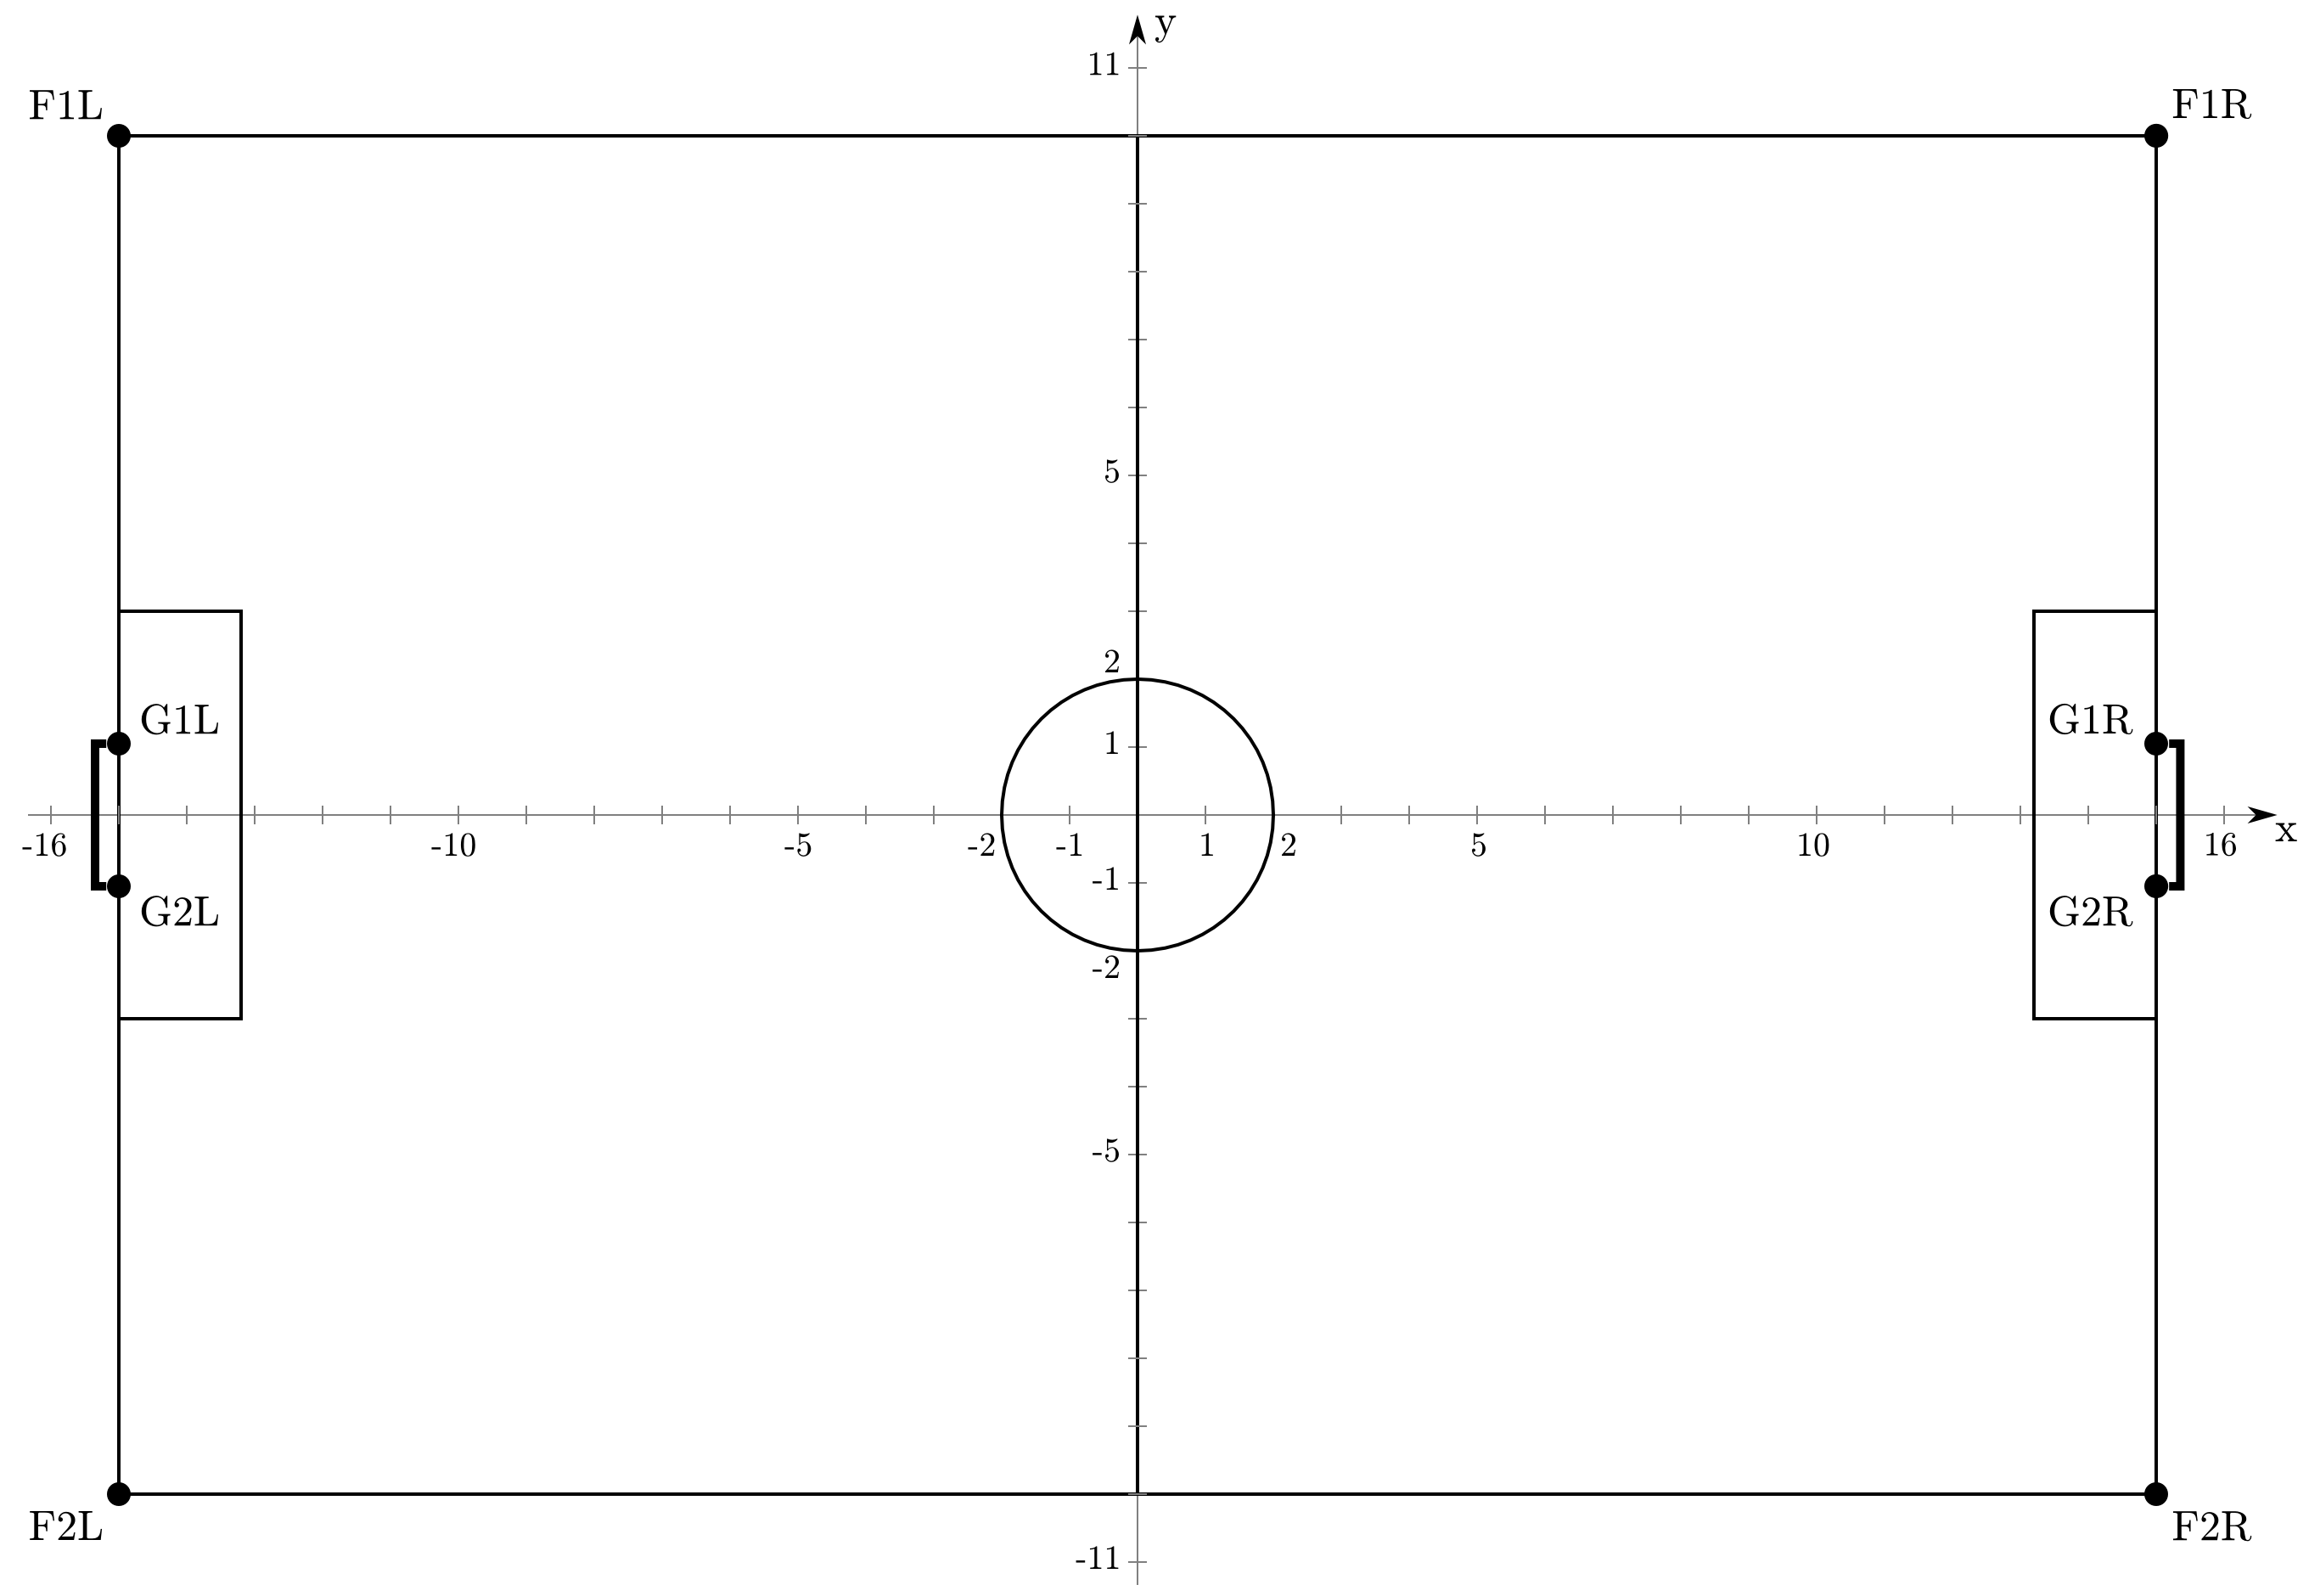
\includegraphics[width=0.9\textwidth]{Chapter2/figures/SoccerSimulation_FieldPlan.png}
  \caption{RoboCup 3D Simulation League Field} 
  \label{fig:SimulationSoccerField}
\end{figure}


\section{Robot Model}
Rcssserver3d comes with the Nao robot model for use by the agents in the soccer simulation. The physical specifications of each model is stored in an \texttt{.rsg} file.The real Nao humanoid robot is manufactured by Aldebaran Robotics in Paris, France. Its height is about 57cm and its weight is around 4.5kg. The simulated model comes with 22 degrees of freedom, which allow Nao to have great mobility. Although, we are discussing about the same robot, there are differences between real and simulated Nao. Real Aldebaran's Nao weight 0.7Kg more than the simulated one. Furthermore, it comes with two cameras attached on its head in the same vertical alignment, maximizing vertically its field of view. These two cameras are not able to work simultaneously but only one at a time. It has also two sonar devices (2x Emitters, 2x Receivers) which are not important to be used in simulated Nao considering its ``advanced'' vision capability. The real model comes with 21 degrees of freedom in contrast to 22 in the simulated Nao, there are two pelvis joints which are coupled together and are not able to move independently. In addition two bumpers are positioned in front of its feet, providing information about possible collisions. Figure~\ref{fig:Naoinsimulationscreen} shows a depiction of the Nao robot model within the into the Rcssserver3d simulation environment.

\begin{figure}[t!]
\centering
  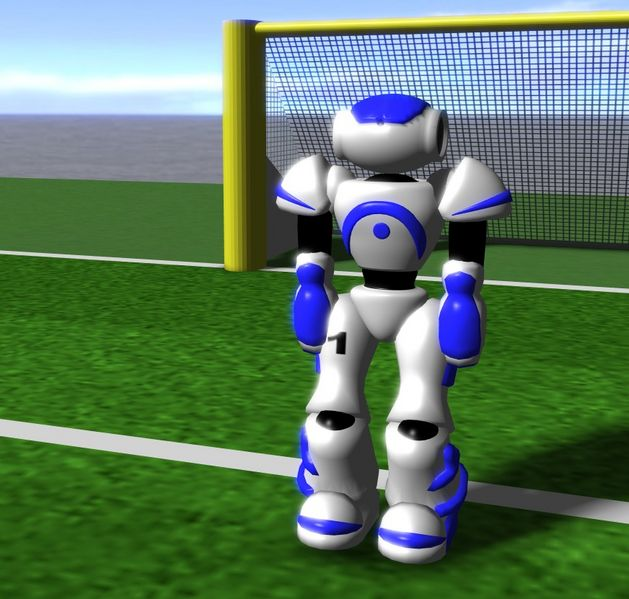
\includegraphics[scale=0.3]{Chapter2/figures/629px-Models-nao.jpg}
  \caption{Nao Robot Model in the Rcssserver3d Soccer Simulation Environment} 
  \label{fig:Naoinsimulationscreen}
\end{figure}

\section{Server}
The SimSpark server hosts the process that manages and advances the simulation. The simulation state is constantly modified through the simulation update loop. Each simulation step corresponds to 20ms of simulated time. Objects in the scene change their state, i.e. one or more of their properties, such as position, speed, angular velocity, etc., due to inherent or external influences. These properties are under the control of a rigid body physical simulation that resolves collisions, applies drag, gravity, etc. Agents that take part in the simulation also modify objects with the help of their effectors, which may move and apply forces to other objects. SimSpark implements a simple internal event model that immediately executes every action received from an agent.


Another responsibility of the server is to keep track of connected agent processes. The SimSpark server exposes a network interface to all agents on TCP port 3100 (default value). In each simulation cycle, the server collects and reports sensor information for each of the sensors of all connected agents. It further carries out received action sequences triggered by the connected agents through their available effectors.
The server does not try to compensate for network latencies or differences in computing resources available to the connected agents. A consequence is that simulations are not reproducible. This means repeated simulations may have a different outcome, depending on network delays or load variations on the machines hosting the agents and the server.


\section{Monitor}

The server can render the simulation itself, depending on its configuration. It implements an internal monitor that omits the network overhead. However, it supports streaming data to remote monitor processes, which take responsibility for rendering the 3D scene for remote viewing.


\subsection{SimSpark Monitor}
The SimSpark monitor is responsible for rendering the current simulation. It connects to a running server instance from which it continuously receives a stream of updates that describe the simulation state, either as full snapshots or as incremental updates.
The format of the data stream the server sends to the monitor is called \textit{Monitor Format}. It is a customizable language used to describe the simulation state in text format.
Apart from describing the pure simulation state, each Monitor Format may provide a mechanism to transfer additional game-specific state. For the soccer simulation, this game-specific state may include, for example, current play mode and goals scored so far. The monitor client itself only renders the pure scene and defers the rendering of the game-specific state to plugins. These plugins are intended to parse the game-specific state and display it as an overlay printed out on screen.



\subsection{Roboviz Monitor}
\textit{RoboViz}~\cite{Roboviz} was created by Justin Stoecker in collaboration with the RoboCup group (RoboCanes) at the University of Miami's Department of Computer Science.
RoboViz is a software program designed to assess and debug agent behaviors in the RoboCup 3D Simulation League. RoboViz is an interactive monitor that renders agent and world state information in a three-dimensional scene. In addition, RoboViz provides programmable drawing and debug functionality to agents that can communicate over a network. The tool facilitates the real-time visualization of agents running concurrently on the SimSpark simulator and provides higher-level analysis and visualization of agent behaviors not currently possible with existing tools. Figure~\ref{fig:Roboviz} shows a visual comparison of the RoboViz and SimSpark Monitors.

\begin{figure}[t!] 
  \begin{center}
    \subfigure{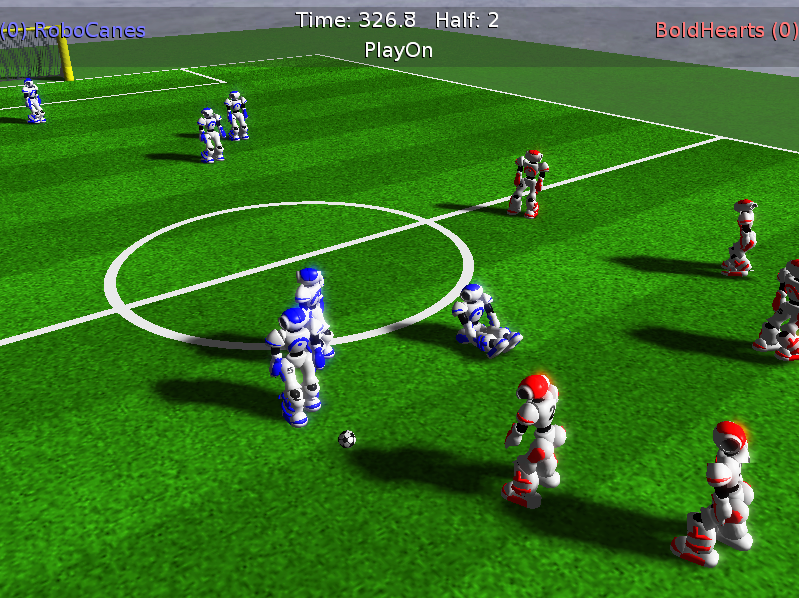
\includegraphics[width=0.4\textwidth]{Chapter2/figures/RobovizMonitor.png}}
    \subfigure{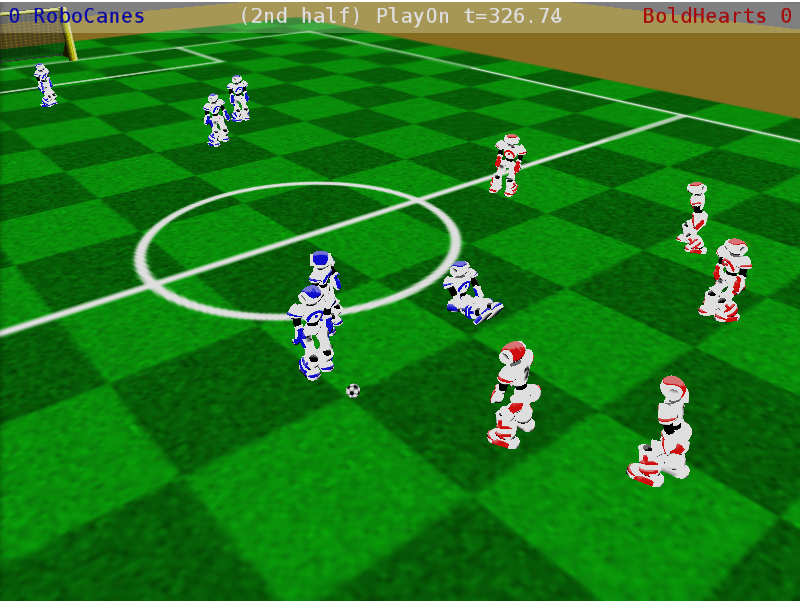
\includegraphics[width=0.4\textwidth]{Chapter2/figures/SimSparkMonitor.png}}
  \end{center}
  \caption{Roboviz (left) vs SimSpark (right) Monitors.}
  \label{fig:Roboviz}
\end{figure}





\section{Perceptors}
Perceptors are the senses of an agent, allowing awareness of the agent's model state and the environment.
The server sends perceptor messages to connected agents via the network protocol at each cycle of the simulation.
There are both general perceptors available in all simulations and soccer perceptors specific to the soccer simulation.



\subsection{General perceptors}

\begin{description}
  \item [HingeJoint Perceptor]
  A hinge joint perceptor receives information about the angle of the corresponding single-axis hinge joint. It contains the identifier \texttt{HJ}, the name of the perceptor, and the position angle of the axis in degrees. A zero angle corresponds to straightly aligned bodies. The position angle of each hinge joint perceptor is sent at each cycle.
Each hinge joint has minimum and maximum limits on its angular position. This varies from hinge to hinge and depends upon the model being used. Nao has 22 hinge joint perceptors; this is the only joint type used in this robot.

 \begin{description}
  \item[{\bf Message format:}]
  \texttt{(HJ (n <name>) (ax <ax>))}
  \item[{\bf Frequency:}]
  Every cycle
   \item[{\bf Noise Model:}] None, however values are truncated to two decimal places, which is equivalent to a uniform error of up to 0.01 degrees.
  \end{description}
  
  
  \item [ForceResistance Perceptor]
  This perceptor informs about the force that acts on a body.  After the identifier \texttt{FRP} and the name of the body, the perceptor message contains two three-dimensional vectors. The first vector describes the coordinates of the point of origin on the body where the force is applied to (in meters) and the second vector is the force vector (magnitude and  direction) of the force applied to this point (in Newtons). This information is just an approximation of the real applied force. The point of origin is calculated as the weighted average of all contact points to which force is applied, while the force vector represents the total force applied to all of these contact points. The perceptor message for force resistance perceptors is sent only in case of a collision of the corresponding body with another simulated object. Nao has two of these perceptors, located below each foot and named \texttt{lf} and \texttt{rf}.
 \begin{description}
  \item[{\bf Message format:}]
  \texttt{(FRP (n <name>) (c <px> <py> <pz>) (f <fx> <fy> <fz>))}
  \item[{\bf Frequency:}]Only in cycles where a body collision occurs
  \item[{\bf Noise Model:}]
  None, however values are truncated to two decimal places, which is equivalent to a uniform error of up to 0.01 meters or Newtons.
  \end{description}


  \item [GyroRate Perceptor]
  The gyro rate perceptor delivers information about the change in orientation of a body. The message contains the \texttt{GYR} identifier, the name of the body to which the gyro perceptor belongs to, and the rates of change of the three rotation (Euler) angles. These values describe the rates of change in orientation of the body during the last cycle, in other words the current angular velocities about the three rotation axes of the corresponding body in degrees per second. To enable keeping track of the orientation of the body, the information to each gyro rate perceptor is sent at each cycle. Nao has one gyro perceptor in the upper torso.
  \begin{description}
  \item[{\bf Message format:}]
  \texttt{(GYR (n <name>) (rt <x> <y> <z>))}
  \item[{\bf Frequency:}]
  Every cycle
  \item[{\bf Noise Model:}]None, however values are truncated to two decimal places, which is equivalent to a uniform error of up to 0.01 degrees.
  \end{description}

  \item [Accelerometer Perceptor]
  This perceptor measures the proper acceleration a body experiences relative to free fall. As a consequence an accelerometer at rest relative to the simulated earth's surface will indicate an acceleration of approximately 1g upwards. To obtain the acceleration due to motion with respect to the earth, this gravity offset should be subtracted. After the identifier \texttt{ACC} and the name of the body, the perceptor message contains a three-dimensional vector with the acceleration values along the three Cartesian axes in $m/s^2$. Nao has one accelerometer in the upper torso.
    \begin{description}
  \item[{\bf Message format:}]
  \texttt{(ACC (n <name>) (a <x> <y> <z>))}
  \item[{\bf Frequency:}]
  Every cycle
  \item[{\bf Noise Model:}]None, however values are truncated to two decimal places, which is equivalent to a uniform error of up to 0.01 $m/s^{2}$.
  \end{description}
\end{description}

\subsection{Soccer perceptors}

\begin{description}
  \item [Vision Perceptor]
The most important perceptor of the Nao robot is the vision perceptor, which delivers information about seen objects in the environment, where objects are either others players, the ball, field lines, or markers on the field. Currently there are eight markers on the field: one at each corner point of the field and one at each goal post. Each player has up to five visible body parts (two arms, two legs, head). Each field line is characterized by two points (starting and ending points). The perceptor message begins with the identifier \texttt{See} and for each visible object it contains a vector described in spherical coordinates. In other words, it contains the distance \texttt{d} (in meters) together with the horizontal \texttt{a1} and vertical \texttt{a2} angles (in degrees) to the center of the object relatively to the focal point of the camera. Nao possesses a restricted vision perceptor at the center of its head. This perceptor's type is \texttt{RestrictedVisionPerceptor}, which limits the field of view to $120^{\circ}$. 

 \begin{description}
  \item[{\bf Message format:}]
  \begin{verbatim}
  (See +(<name> (pol <d> <a1> <a2>))
  +(P (team <name>) (id <ID>) +(<bodypart> (pol <d> <a1> <a2>)))
  +(L (pol <d> <a1> <a2>)(pol <d> <a1> <a2>)) )\end{verbatim}
  \item[{\bf Frequency:}]
 Every third cycle (60ms)
  \item[{\bf Noise Model:}] Calibration error (a fixed offset of around $\pm0.004m$ in each of $x/y/z$ axes), zero-mean Gaussian noise, and values truncated to two decimal places, which is equivalent to a uniform error of up to 0.01 meters or degrees.
  \end{description}


  \item [Hear Perceptor]
The agent processes are not allowed to communicate with each other directly, but the agents may exchange messages via the simulation server. For this purpose agents are equipped with the so-called hear perceptor, which serves as an aural sensor and receives messages shouted by other players. A hear perceptor message begins with the \texttt{hear} identifier, followed by the simulation time at which the given message was heard in seconds, either a relative horizontal direction in degrees indicating where the sound originated or \texttt{self} indicating that the player is hearing their own shouted message, and finally the message itself in plain ASCII text (parentheses cannot be part of the message). Messages should not have a length of more than 20 ASCII characters. Messages shouted from beyond a maximal distance (currently 50 meters) cannot be heard. Most important restriction is that only one message can be heard at any given time and messages from the same team can be heard only every other cycle. All unheard messages are lost. Thus, the maximum communication bandwidth is 20 ASCII characters every $40ms$.
  \begin{description}
  \item[{\bf Message format:}]
  \texttt{(hear <time> self/<direction> <message>)}
  \item[{\bf Frequency:}]
  Only in cycles, where a message is heard
  \end{description}
  
  
    \item [GameState Perceptor]
  The game state perceptor delivers information about the actual state of the soccer game environment. A game state message begins with the \texttt{GS} identifier, followed by two pieces of game state information: the actual play time and the current play mode (\texttt{BeforeKickOff}, \texttt{PlayOn}, \texttt{KickOff\_Left}, \texttt{KickOff\_Right}, \texttt{GoalLeft}, \texttt{GoalRight}, \texttt{corner\_kick\_left}, \texttt{corner\_kick\_right}, \texttt{KickInLeft}, \texttt{KickInRight}, \texttt{goal\_kick\_left}, \texttt{goal\_kick\_right}). Play time starts at $0$ at the kickoff of the first half and at $300$ at the kickoff of the second half and is given in seconds with a precision of two decimal places.
  \begin{description}
  \item[{\bf Message format:}]
  \texttt{(GS (t <time>) (pm <playmode>))}
  \item[{\bf Frequency:}]
 Every cycle
  \end{description}
\end{description}
\section{Effectors}

Effectors allow agents to perform actions within the simulation. Agents control them by sending messages to the server and the server changes the game state accordingly.
Effector control messages are sent via the network protocol. There are both general effectors that apply to all simulations, and soccer effectors that are specific to the soccer simulation.
\subsection{General Effectors}
\begin{description}


\item [Create Effector]
When an agent initially connects to the server, it is invisible and cannot affect a simulation in any meaningful way. It only possesses a so-called CreateEffector, whose message begins with the \texttt{scene} identifier. An agent uses this effector to advice the server to construct the physical representation and all further effectors and perceptors of the agent in the simulation environment according to a scene description file it passes as a parameter.
  \begin{description}
  \item[{\bf Message format:}]
  \texttt{(scene <filename>)}
  \item[{\bf Frequency:}]
  Only once
  \end{description}

  \item [HingeJoint Effector]
Effector for all axes with a single degree of freedom. The first parameter is the name of the axis. The second parameter is a speed value given in degrees per second. Setting a speed value on a hinge means that the speed will be maintained until a new value is provided. Even if the hinge meets its extremity, it will bounce around the extremity until a new speed value is requested.
  \begin{description}
  \item[{\bf Message format:}]
  \texttt{(<name> <ax>)}
  \item[{\bf Frequency:}]
  Once per cycle maximum
  \end{description}

  \item [Synchronize Effector]
  Agents running in Agent Sync Mode must send this command at the end of each simulation cycle. Note that the server ignores this command, if it is received in Real-Time Mode, so it is safe to configure agents to always append this command to responses.
  \begin{description}
  \item[{\bf Message format:}]
  \texttt{(syn)}
  \item[{\bf Frequency:}]
  Every cycle
  \end{description}

\end{description}




\subsection{Soccer Effectors}


\begin{description}


  \item [Init Effector]
  The init command is sent once for each agent, after the create effector message has been sent. The init effector registers the agent as a member of a team with a specific player number, both of which are passed as arguments in the init effector message after the identifier \texttt{init}. All players of one team must use the same team name and different player numbers. When an agent connects to the server, he must first send a \texttt{CreateEffector} message followed by an \texttt{InitEffector} message in order to initialize himself into the soccer field.
  \begin{description}
  \item[{\bf Message format:}]  
  \texttt{(init (unum <playernumber>) (teamname <teamname>) )}
  \item[{\bf Frequency:}]
  Only once
  \end{description}



  \item [Beam Effector]
  The beam effector allows a player to position itself anywhere on the field only before any kick-off (at the start of each half or right after a goal has been scored). After the \texttt{beam} identifier, the \texttt{x} and \texttt{y} coordinates define the position on the field with respect to the field's coordinate system in meters, where $(0,0)$ is the absolute center of the field. The \texttt{rot} argument specifies the facing angle of the player in degrees. A value of 0 points towards the positive x-axis, whereas a value of 90 points to positive y-axis.
  \begin{description}
  \item[{\bf Message format:}]  
  \texttt{(beam <x> <y> <rot>)}
  \item[{\bf Frequency:}]
  Once before each kick-off
  \end{description}



  \item [Say Effector]
  The say effector permits communication among agents by broadcasting messages in plain ASCII text (20 characters maximum). In order to say something, the following command has to be employed.
  \begin{description}
  \item[{\bf Message format:}]
  \texttt{(say <message>)}
  \item[{\bf Frequency:}]
  Once per cycle maximum
  \end{description}

\end{description}
